\documentclass[]{article}
\usepackage{lmodern}
\usepackage{amssymb,amsmath}
\usepackage{ifxetex,ifluatex}
\usepackage{fixltx2e} % provides \textsubscript
\ifnum 0\ifxetex 1\fi\ifluatex 1\fi=0 % if pdftex
  \usepackage[T1]{fontenc}
  \usepackage[utf8]{inputenc}
\else % if luatex or xelatex
  \ifxetex
    \usepackage{mathspec}
  \else
    \usepackage{fontspec}
  \fi
  \defaultfontfeatures{Ligatures=TeX,Scale=MatchLowercase}
\fi
% use upquote if available, for straight quotes in verbatim environments
\IfFileExists{upquote.sty}{\usepackage{upquote}}{}
% use microtype if available
\IfFileExists{microtype.sty}{%
\usepackage{microtype}
\UseMicrotypeSet[protrusion]{basicmath} % disable protrusion for tt fonts
}{}
\usepackage[margin=1in]{geometry}
\usepackage{hyperref}
\hypersetup{unicode=true,
            pdfborder={0 0 0},
            breaklinks=true}
\urlstyle{same}  % don't use monospace font for urls
\usepackage{color}
\usepackage{fancyvrb}
\newcommand{\VerbBar}{|}
\newcommand{\VERB}{\Verb[commandchars=\\\{\}]}
\DefineVerbatimEnvironment{Highlighting}{Verbatim}{commandchars=\\\{\}}
% Add ',fontsize=\small' for more characters per line
\usepackage{framed}
\definecolor{shadecolor}{RGB}{248,248,248}
\newenvironment{Shaded}{\begin{snugshade}}{\end{snugshade}}
\newcommand{\KeywordTok}[1]{\textcolor[rgb]{0.13,0.29,0.53}{\textbf{#1}}}
\newcommand{\DataTypeTok}[1]{\textcolor[rgb]{0.13,0.29,0.53}{#1}}
\newcommand{\DecValTok}[1]{\textcolor[rgb]{0.00,0.00,0.81}{#1}}
\newcommand{\BaseNTok}[1]{\textcolor[rgb]{0.00,0.00,0.81}{#1}}
\newcommand{\FloatTok}[1]{\textcolor[rgb]{0.00,0.00,0.81}{#1}}
\newcommand{\ConstantTok}[1]{\textcolor[rgb]{0.00,0.00,0.00}{#1}}
\newcommand{\CharTok}[1]{\textcolor[rgb]{0.31,0.60,0.02}{#1}}
\newcommand{\SpecialCharTok}[1]{\textcolor[rgb]{0.00,0.00,0.00}{#1}}
\newcommand{\StringTok}[1]{\textcolor[rgb]{0.31,0.60,0.02}{#1}}
\newcommand{\VerbatimStringTok}[1]{\textcolor[rgb]{0.31,0.60,0.02}{#1}}
\newcommand{\SpecialStringTok}[1]{\textcolor[rgb]{0.31,0.60,0.02}{#1}}
\newcommand{\ImportTok}[1]{#1}
\newcommand{\CommentTok}[1]{\textcolor[rgb]{0.56,0.35,0.01}{\textit{#1}}}
\newcommand{\DocumentationTok}[1]{\textcolor[rgb]{0.56,0.35,0.01}{\textbf{\textit{#1}}}}
\newcommand{\AnnotationTok}[1]{\textcolor[rgb]{0.56,0.35,0.01}{\textbf{\textit{#1}}}}
\newcommand{\CommentVarTok}[1]{\textcolor[rgb]{0.56,0.35,0.01}{\textbf{\textit{#1}}}}
\newcommand{\OtherTok}[1]{\textcolor[rgb]{0.56,0.35,0.01}{#1}}
\newcommand{\FunctionTok}[1]{\textcolor[rgb]{0.00,0.00,0.00}{#1}}
\newcommand{\VariableTok}[1]{\textcolor[rgb]{0.00,0.00,0.00}{#1}}
\newcommand{\ControlFlowTok}[1]{\textcolor[rgb]{0.13,0.29,0.53}{\textbf{#1}}}
\newcommand{\OperatorTok}[1]{\textcolor[rgb]{0.81,0.36,0.00}{\textbf{#1}}}
\newcommand{\BuiltInTok}[1]{#1}
\newcommand{\ExtensionTok}[1]{#1}
\newcommand{\PreprocessorTok}[1]{\textcolor[rgb]{0.56,0.35,0.01}{\textit{#1}}}
\newcommand{\AttributeTok}[1]{\textcolor[rgb]{0.77,0.63,0.00}{#1}}
\newcommand{\RegionMarkerTok}[1]{#1}
\newcommand{\InformationTok}[1]{\textcolor[rgb]{0.56,0.35,0.01}{\textbf{\textit{#1}}}}
\newcommand{\WarningTok}[1]{\textcolor[rgb]{0.56,0.35,0.01}{\textbf{\textit{#1}}}}
\newcommand{\AlertTok}[1]{\textcolor[rgb]{0.94,0.16,0.16}{#1}}
\newcommand{\ErrorTok}[1]{\textcolor[rgb]{0.64,0.00,0.00}{\textbf{#1}}}
\newcommand{\NormalTok}[1]{#1}
\usepackage{graphicx,grffile}
\makeatletter
\def\maxwidth{\ifdim\Gin@nat@width>\linewidth\linewidth\else\Gin@nat@width\fi}
\def\maxheight{\ifdim\Gin@nat@height>\textheight\textheight\else\Gin@nat@height\fi}
\makeatother
% Scale images if necessary, so that they will not overflow the page
% margins by default, and it is still possible to overwrite the defaults
% using explicit options in \includegraphics[width, height, ...]{}
\setkeys{Gin}{width=\maxwidth,height=\maxheight,keepaspectratio}
\IfFileExists{parskip.sty}{%
\usepackage{parskip}
}{% else
\setlength{\parindent}{0pt}
\setlength{\parskip}{6pt plus 2pt minus 1pt}
}
\setlength{\emergencystretch}{3em}  % prevent overfull lines
\providecommand{\tightlist}{%
  \setlength{\itemsep}{0pt}\setlength{\parskip}{0pt}}
\setcounter{secnumdepth}{0}
% Redefines (sub)paragraphs to behave more like sections
\ifx\paragraph\undefined\else
\let\oldparagraph\paragraph
\renewcommand{\paragraph}[1]{\oldparagraph{#1}\mbox{}}
\fi
\ifx\subparagraph\undefined\else
\let\oldsubparagraph\subparagraph
\renewcommand{\subparagraph}[1]{\oldsubparagraph{#1}\mbox{}}
\fi

%%% Use protect on footnotes to avoid problems with footnotes in titles
\let\rmarkdownfootnote\footnote%
\def\footnote{\protect\rmarkdownfootnote}

%%% Change title format to be more compact
\usepackage{titling}

% Create subtitle command for use in maketitle
\newcommand{\subtitle}[1]{
  \posttitle{
    \begin{center}\large#1\end{center}
    }
}

\setlength{\droptitle}{-2em}

  \title{}
    \pretitle{\vspace{\droptitle}}
  \posttitle{}
    \author{}
    \preauthor{}\postauthor{}
    \date{}
    \predate{}\postdate{}
  

\begin{document}

\begin{Shaded}
\begin{Highlighting}[]
\NormalTok{knitr}\OperatorTok{::}\NormalTok{opts_chunk}\OperatorTok{$}\KeywordTok{set}\NormalTok{(}\DataTypeTok{echo =} \OtherTok{TRUE}\NormalTok{)}

\KeywordTok{library}\NormalTok{(mvtnorm)}
\KeywordTok{library}\NormalTok{(afex)}
\KeywordTok{library}\NormalTok{(emmeans)}
\KeywordTok{library}\NormalTok{(ggplot2)}
\KeywordTok{library}\NormalTok{(gridExtra)}
\KeywordTok{library}\NormalTok{(reshape2)}
\KeywordTok{library}\NormalTok{(pwr)}

\CommentTok{# Install functions from GitHub by running the code below:}
\KeywordTok{source}\NormalTok{(}\StringTok{"https://raw.githubusercontent.com/Lakens/ANOVA_power_simulation/master/helper_functions/plot_power_2x2_within.R"}\NormalTok{)}
\end{Highlighting}
\end{Shaded}

\subsection{Power curves}\label{power-curves}

Power is calculated for a specific value of an effect size, alpha level,
and sample size. Because you often do not know the true effect size, it
often makes more sense to think of the power curve as a function of the
size of the effect. Although power curves can be calculated based on
simulations for any design, we will use the analytic solution to
calculate the power of ANOVA designs because these calculations are much
faster. The basic approach is to calculate power for a specific pattern
of means, a specific effect size, a given alpha level, and a specific
pattern of correlations. This is one example:

\begin{Shaded}
\begin{Highlighting}[]
\CommentTok{#2x2 design}
\NormalTok{mu =}\StringTok{ }\KeywordTok{c}\NormalTok{(}\DecValTok{0}\NormalTok{,}\DecValTok{0}\NormalTok{,}\DecValTok{0}\NormalTok{,}\FloatTok{0.5}\NormalTok{)}
\NormalTok{m_A =}\StringTok{ }\DecValTok{2} \CommentTok{# 2 levels of factor A}
\NormalTok{m_B =}\StringTok{ }\DecValTok{2}  \CommentTok{# 2 levels of factor B}
\NormalTok{sigma =}\StringTok{ }\DecValTok{1} 
\NormalTok{n =}\StringTok{ }\DecValTok{20}
\NormalTok{rho_A =}\StringTok{ }\FloatTok{0.5}
\NormalTok{rho_B =}\StringTok{ }\FloatTok{0.5}
\NormalTok{rho_AB =}\StringTok{ }\FloatTok{0.5}
\NormalTok{alpha =}\StringTok{ }\FloatTok{0.05}

\NormalTok{power_res <-}\StringTok{ }\KeywordTok{power_2x2_within}\NormalTok{(}\DataTypeTok{mu =}\NormalTok{ mu, }
                              \DataTypeTok{m_A =}\NormalTok{ m_A, }
                              \DataTypeTok{m_B =}\NormalTok{ m_B, }
                              \DataTypeTok{sigma =}\NormalTok{ sigma, }
                              \DataTypeTok{n =}\NormalTok{ n, }
                              \DataTypeTok{rho_A =}\NormalTok{ rho_A, }
                              \DataTypeTok{rho_B =}\NormalTok{ rho_B, }
                              \DataTypeTok{rho_AB =}\NormalTok{ rho_AB, }
                              \DataTypeTok{alpha =}\NormalTok{ alpha)}

\NormalTok{power_res}\OperatorTok{$}\NormalTok{pow_A}
\end{Highlighting}
\end{Shaded}

\begin{verbatim}
## [1] 0.3235926
\end{verbatim}

\begin{Shaded}
\begin{Highlighting}[]
\NormalTok{power_res}\OperatorTok{$}\NormalTok{pow_B}
\end{Highlighting}
\end{Shaded}

\begin{verbatim}
## [1] 0.3235926
\end{verbatim}

\begin{Shaded}
\begin{Highlighting}[]
\NormalTok{power_res}\OperatorTok{$}\NormalTok{pow_AB}
\end{Highlighting}
\end{Shaded}

\begin{verbatim}
## [1] 0.5645044
\end{verbatim}

We can make these calculations for a range of sample sizes, to get a
power curve. We created a simple function that performs these
calculations across a range of sample sizes (from n = 2 to max\_, a
variable you can specify in the function).

\begin{Shaded}
\begin{Highlighting}[]
\NormalTok{p_a <-}\StringTok{ }\KeywordTok{plot_power_2x2_within}\NormalTok{(}\DataTypeTok{mu =} \KeywordTok{c}\NormalTok{(}\DecValTok{0}\NormalTok{,}\DecValTok{0}\NormalTok{,}\DecValTok{0}\NormalTok{,}\FloatTok{0.5}\NormalTok{), }
                      \DataTypeTok{m_A =} \DecValTok{2}\NormalTok{, }
                      \DataTypeTok{m_B =} \DecValTok{2}\NormalTok{, }
                      \DataTypeTok{sigma =} \DecValTok{1}\NormalTok{, }
                      \DataTypeTok{rho_A =} \FloatTok{0.5}\NormalTok{, }
                      \DataTypeTok{rho_B =} \FloatTok{0.5}\NormalTok{, }
                      \DataTypeTok{rho_AB =} \FloatTok{0.5}\NormalTok{, }
                      \DataTypeTok{alpha =} \FloatTok{0.05}\NormalTok{,}
\NormalTok{                      max_n <-}\StringTok{ }\DecValTok{50}\NormalTok{)}

\KeywordTok{grid.arrange}\NormalTok{(p_a}\OperatorTok{$}\NormalTok{p1, p_a}\OperatorTok{$}\NormalTok{p2, p_a}\OperatorTok{$}\NormalTok{p3, }\DataTypeTok{nrow =} \DecValTok{1}\NormalTok{)}
\end{Highlighting}
\end{Shaded}

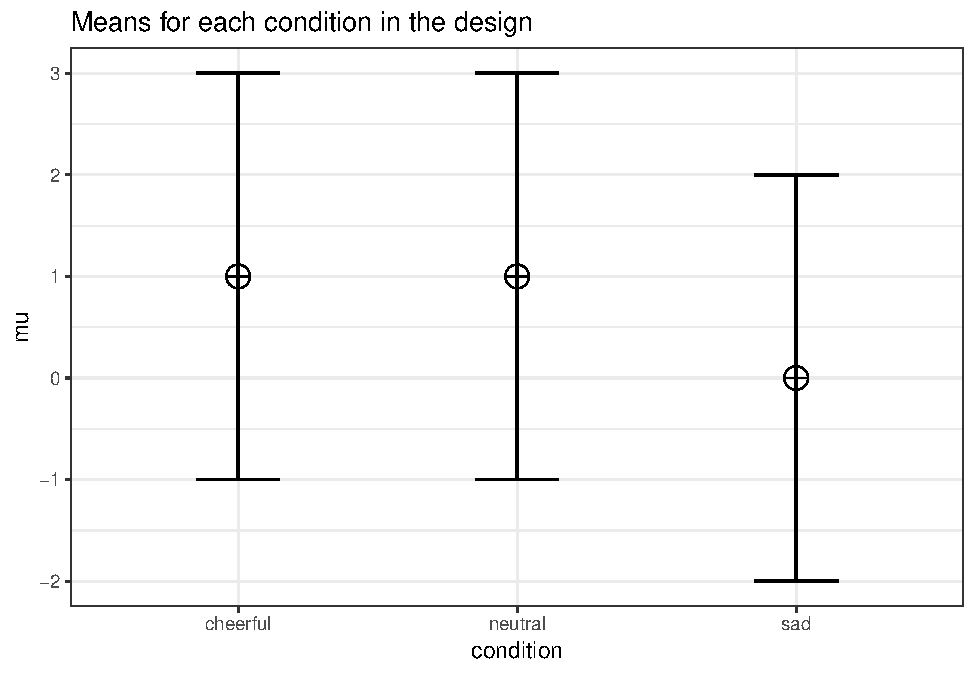
\includegraphics{4.4_power_curves_2x2_within_files/figure-latex/unnamed-chunk-3-1.pdf}

\section{Explore increase in effect size for moderated
interactions.}\label{explore-increase-in-effect-size-for-moderated-interactions.}

The design has means 0, 0, 0, 0, with one cell increasing by 0.1, up to
0, 0, 0, 0.5. The standard deviation is set to 1. The correlation
between all variables is 0.5.

\begin{Shaded}
\begin{Highlighting}[]
\NormalTok{p_a <-}\StringTok{ }\KeywordTok{plot_power_2x2_within}\NormalTok{(}\DataTypeTok{mu =} \KeywordTok{c}\NormalTok{(}\DecValTok{0}\NormalTok{,}\DecValTok{0}\NormalTok{,}\DecValTok{0}\NormalTok{,}\FloatTok{0.0}\NormalTok{), }
                      \DataTypeTok{m_A =} \DecValTok{2}\NormalTok{, }
                      \DataTypeTok{m_B =} \DecValTok{2}\NormalTok{, }
                      \DataTypeTok{sigma =} \DecValTok{1}\NormalTok{, }
                      \DataTypeTok{rho_A =} \FloatTok{0.5}\NormalTok{, }
                      \DataTypeTok{rho_B =} \FloatTok{0.5}\NormalTok{, }
                      \DataTypeTok{rho_AB =} \FloatTok{0.5}\NormalTok{, }
                      \DataTypeTok{alpha =} \FloatTok{0.05}\NormalTok{,}
\NormalTok{                      max_n <-}\StringTok{ }\DecValTok{100}\NormalTok{)}

\NormalTok{p_b <-}\StringTok{ }\KeywordTok{plot_power_2x2_within}\NormalTok{(}\DataTypeTok{mu =} \KeywordTok{c}\NormalTok{(}\DecValTok{0}\NormalTok{,}\DecValTok{0}\NormalTok{,}\DecValTok{0}\NormalTok{,}\FloatTok{0.1}\NormalTok{), }
                      \DataTypeTok{m_A =} \DecValTok{2}\NormalTok{, }
                      \DataTypeTok{m_B =} \DecValTok{2}\NormalTok{, }
                      \DataTypeTok{sigma =} \DecValTok{1}\NormalTok{, }
                      \DataTypeTok{rho_A =} \FloatTok{0.5}\NormalTok{, }
                      \DataTypeTok{rho_B =} \FloatTok{0.5}\NormalTok{, }
                      \DataTypeTok{rho_AB =} \FloatTok{0.5}\NormalTok{, }
                      \DataTypeTok{alpha =} \FloatTok{0.05}\NormalTok{,}
\NormalTok{                      max_n <-}\StringTok{ }\DecValTok{100}\NormalTok{)}

\NormalTok{p_c <-}\StringTok{ }\KeywordTok{plot_power_2x2_within}\NormalTok{(}\DataTypeTok{mu =} \KeywordTok{c}\NormalTok{(}\DecValTok{0}\NormalTok{,}\DecValTok{0}\NormalTok{,}\DecValTok{0}\NormalTok{,}\FloatTok{0.2}\NormalTok{), }
                      \DataTypeTok{m_A =} \DecValTok{2}\NormalTok{, }
                      \DataTypeTok{m_B =} \DecValTok{2}\NormalTok{, }
                      \DataTypeTok{sigma =} \DecValTok{1}\NormalTok{, }
                      \DataTypeTok{rho_A =} \FloatTok{0.5}\NormalTok{, }
                      \DataTypeTok{rho_B =} \FloatTok{0.5}\NormalTok{, }
                      \DataTypeTok{rho_AB =} \FloatTok{0.5}\NormalTok{, }
                      \DataTypeTok{alpha =} \FloatTok{0.05}\NormalTok{,}
\NormalTok{                      max_n <-}\StringTok{ }\DecValTok{100}\NormalTok{)}

\NormalTok{p_d <-}\StringTok{ }\KeywordTok{plot_power_2x2_within}\NormalTok{(}\DataTypeTok{mu =} \KeywordTok{c}\NormalTok{(}\DecValTok{0}\NormalTok{,}\DecValTok{0}\NormalTok{,}\DecValTok{0}\NormalTok{,}\FloatTok{0.3}\NormalTok{), }
                      \DataTypeTok{m_A =} \DecValTok{2}\NormalTok{, }
                      \DataTypeTok{m_B =} \DecValTok{2}\NormalTok{, }
                      \DataTypeTok{sigma =} \DecValTok{1}\NormalTok{, }
                      \DataTypeTok{rho_A =} \FloatTok{0.5}\NormalTok{, }
                      \DataTypeTok{rho_B =} \FloatTok{0.5}\NormalTok{, }
                      \DataTypeTok{rho_AB =} \FloatTok{0.5}\NormalTok{, }
                      \DataTypeTok{alpha =} \FloatTok{0.05}\NormalTok{,}
\NormalTok{                      max_n <-}\StringTok{ }\DecValTok{100}\NormalTok{)}

\NormalTok{p_e <-}\StringTok{ }\KeywordTok{plot_power_2x2_within}\NormalTok{(}\DataTypeTok{mu =} \KeywordTok{c}\NormalTok{(}\DecValTok{0}\NormalTok{,}\DecValTok{0}\NormalTok{,}\DecValTok{0}\NormalTok{,}\FloatTok{0.4}\NormalTok{), }
                      \DataTypeTok{m_A =} \DecValTok{2}\NormalTok{, }
                      \DataTypeTok{m_B =} \DecValTok{2}\NormalTok{, }
                      \DataTypeTok{sigma =} \DecValTok{1}\NormalTok{, }
                      \DataTypeTok{rho_A =} \FloatTok{0.5}\NormalTok{, }
                      \DataTypeTok{rho_B =} \FloatTok{0.5}\NormalTok{, }
                      \DataTypeTok{rho_AB =} \FloatTok{0.5}\NormalTok{, }
                      \DataTypeTok{alpha =} \FloatTok{0.05}\NormalTok{,}
\NormalTok{                      max_n <-}\StringTok{ }\DecValTok{100}\NormalTok{)}

\NormalTok{p_f <-}\StringTok{ }\KeywordTok{plot_power_2x2_within}\NormalTok{(}\DataTypeTok{mu =} \KeywordTok{c}\NormalTok{(}\DecValTok{0}\NormalTok{,}\DecValTok{0}\NormalTok{,}\DecValTok{0}\NormalTok{,}\FloatTok{0.5}\NormalTok{), }
                      \DataTypeTok{m_A =} \DecValTok{2}\NormalTok{, }
                      \DataTypeTok{m_B =} \DecValTok{2}\NormalTok{, }
                      \DataTypeTok{sigma =} \DecValTok{1}\NormalTok{, }
                      \DataTypeTok{rho_A =} \FloatTok{0.5}\NormalTok{, }
                      \DataTypeTok{rho_B =} \FloatTok{0.5}\NormalTok{, }
                      \DataTypeTok{rho_AB =} \FloatTok{0.5}\NormalTok{, }
                      \DataTypeTok{alpha =} \FloatTok{0.05}\NormalTok{,}
\NormalTok{                      max_n <-}\StringTok{ }\DecValTok{100}\NormalTok{)}

\CommentTok{# Create long format dataframe }
\NormalTok{zzz <-}\StringTok{ }\KeywordTok{rbind}\NormalTok{(p_a}\OperatorTok{$}\NormalTok{power_df, p_b}\OperatorTok{$}\NormalTok{power_df, p_c}\OperatorTok{$}\NormalTok{power_df, p_d}\OperatorTok{$}\NormalTok{power_df, p_e}\OperatorTok{$}\NormalTok{power_df, p_f}\OperatorTok{$}\NormalTok{power_df)}
\NormalTok{zzz <-}\StringTok{ }\KeywordTok{cbind}\NormalTok{(zzz,}\KeywordTok{seq}\NormalTok{(}\DecValTok{1}\NormalTok{,}\KeywordTok{length}\NormalTok{(zzz}\OperatorTok{$}\NormalTok{design)))}
\KeywordTok{colnames}\NormalTok{(zzz)[}\DecValTok{1}\NormalTok{] <-}\StringTok{ "design"}
\KeywordTok{colnames}\NormalTok{(zzz)[}\DecValTok{6}\NormalTok{] <-}\StringTok{ "ID"}
\NormalTok{zzz <-}\StringTok{ }\KeywordTok{melt}\NormalTok{(zzz, }\DataTypeTok{id.vars =} \KeywordTok{c}\NormalTok{(}\StringTok{"ID"}\NormalTok{, }\StringTok{"design"}\NormalTok{, }\StringTok{"n_vec"}\NormalTok{), }\DataTypeTok{measure.vars =} \KeywordTok{c}\NormalTok{(}\StringTok{"power_A"}\NormalTok{, }\StringTok{"power_B"}\NormalTok{, }\StringTok{"power_AB"}\NormalTok{))}

\CommentTok{# Plot data using facets, split by factors and interaction, and design}
\KeywordTok{ggplot}\NormalTok{(}\DataTypeTok{data=}\NormalTok{zzz, }\KeywordTok{aes}\NormalTok{(}\DataTypeTok{x =}\NormalTok{ n_vec, }\DataTypeTok{y =}\NormalTok{ value)) }\OperatorTok{+}
\StringTok{  }\KeywordTok{geom_line}\NormalTok{( }\DataTypeTok{size=}\FloatTok{1.5}\NormalTok{) }\OperatorTok{+}
\StringTok{  }\KeywordTok{scale_x_continuous}\NormalTok{(}\DataTypeTok{limits =} \KeywordTok{c}\NormalTok{(}\DecValTok{0}\NormalTok{, }\KeywordTok{max}\NormalTok{(zzz}\OperatorTok{$}\NormalTok{n_vec))) }\OperatorTok{+}\StringTok{ }
\StringTok{  }\KeywordTok{scale_y_continuous}\NormalTok{(}\DataTypeTok{limits =} \KeywordTok{c}\NormalTok{(}\DecValTok{0}\NormalTok{, }\DecValTok{100}\NormalTok{)) }\OperatorTok{+}
\StringTok{  }\KeywordTok{theme_bw}\NormalTok{() }\OperatorTok{+}
\StringTok{  }\KeywordTok{labs}\NormalTok{(}\DataTypeTok{x=}\StringTok{"Sample size"}\NormalTok{, }\DataTypeTok{y =} \StringTok{"Power"}\NormalTok{) }\OperatorTok{+}
\StringTok{  }\KeywordTok{facet_grid}\NormalTok{(design}\OperatorTok{~}\NormalTok{variable)}
\end{Highlighting}
\end{Shaded}

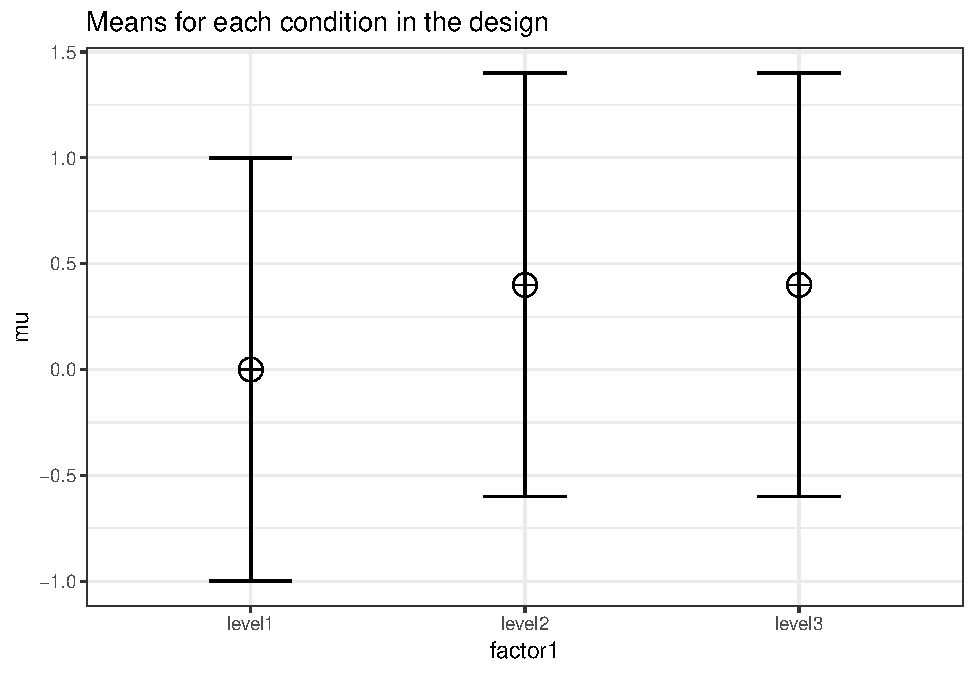
\includegraphics{4.4_power_curves_2x2_within_files/figure-latex/unnamed-chunk-4-1.pdf}

\section{Explore increase in effect size for cross-over
interactions.}\label{explore-increase-in-effect-size-for-cross-over-interactions.}

The design has means 0, 0, 0, 0, with two cells increasing by 0.1, up to
0.5, 0, 0, 0.5. The standard deviation is set to 1. The correlation
between all variables is 0.5.

\begin{Shaded}
\begin{Highlighting}[]
\NormalTok{p_a <-}\StringTok{ }\KeywordTok{plot_power_2x2_within}\NormalTok{(}\DataTypeTok{mu =} \KeywordTok{c}\NormalTok{(}\DecValTok{0}\NormalTok{,}\DecValTok{0}\NormalTok{,}\DecValTok{0}\NormalTok{,}\FloatTok{0.0}\NormalTok{), }
                      \DataTypeTok{m_A =} \DecValTok{2}\NormalTok{, }
                      \DataTypeTok{m_B =} \DecValTok{2}\NormalTok{, }
                      \DataTypeTok{sigma =} \DecValTok{1}\NormalTok{, }
                      \DataTypeTok{rho_A =} \FloatTok{0.5}\NormalTok{, }
                      \DataTypeTok{rho_B =} \FloatTok{0.5}\NormalTok{, }
                      \DataTypeTok{rho_AB =} \FloatTok{0.5}\NormalTok{, }
                      \DataTypeTok{alpha =} \FloatTok{0.05}\NormalTok{,}
\NormalTok{                      max_n <-}\StringTok{ }\DecValTok{100}\NormalTok{)}

\NormalTok{p_b <-}\StringTok{ }\KeywordTok{plot_power_2x2_within}\NormalTok{(}\DataTypeTok{mu =} \KeywordTok{c}\NormalTok{(}\FloatTok{0.1}\NormalTok{,}\DecValTok{0}\NormalTok{,}\DecValTok{0}\NormalTok{,}\FloatTok{0.1}\NormalTok{), }
                      \DataTypeTok{m_A =} \DecValTok{2}\NormalTok{, }
                      \DataTypeTok{m_B =} \DecValTok{2}\NormalTok{, }
                      \DataTypeTok{sigma =} \DecValTok{1}\NormalTok{, }
                      \DataTypeTok{rho_A =} \FloatTok{0.5}\NormalTok{, }
                      \DataTypeTok{rho_B =} \FloatTok{0.5}\NormalTok{, }
                      \DataTypeTok{rho_AB =} \FloatTok{0.5}\NormalTok{, }
                      \DataTypeTok{alpha =} \FloatTok{0.05}\NormalTok{,}
\NormalTok{                      max_n <-}\StringTok{ }\DecValTok{100}\NormalTok{)}

\NormalTok{p_c <-}\StringTok{ }\KeywordTok{plot_power_2x2_within}\NormalTok{(}\DataTypeTok{mu =} \KeywordTok{c}\NormalTok{(}\FloatTok{0.2}\NormalTok{,}\DecValTok{0}\NormalTok{,}\DecValTok{0}\NormalTok{,}\FloatTok{0.2}\NormalTok{), }
                      \DataTypeTok{m_A =} \DecValTok{2}\NormalTok{, }
                      \DataTypeTok{m_B =} \DecValTok{2}\NormalTok{, }
                      \DataTypeTok{sigma =} \DecValTok{1}\NormalTok{, }
                      \DataTypeTok{rho_A =} \FloatTok{0.5}\NormalTok{, }
                      \DataTypeTok{rho_B =} \FloatTok{0.5}\NormalTok{, }
                      \DataTypeTok{rho_AB =} \FloatTok{0.5}\NormalTok{, }
                      \DataTypeTok{alpha =} \FloatTok{0.05}\NormalTok{,}
\NormalTok{                      max_n <-}\StringTok{ }\DecValTok{100}\NormalTok{)}

\NormalTok{p_d <-}\StringTok{ }\KeywordTok{plot_power_2x2_within}\NormalTok{(}\DataTypeTok{mu =} \KeywordTok{c}\NormalTok{(}\FloatTok{0.3}\NormalTok{,}\DecValTok{0}\NormalTok{,}\DecValTok{0}\NormalTok{,}\FloatTok{0.3}\NormalTok{), }
                      \DataTypeTok{m_A =} \DecValTok{2}\NormalTok{, }
                      \DataTypeTok{m_B =} \DecValTok{2}\NormalTok{, }
                      \DataTypeTok{sigma =} \DecValTok{1}\NormalTok{, }
                      \DataTypeTok{rho_A =} \FloatTok{0.5}\NormalTok{, }
                      \DataTypeTok{rho_B =} \FloatTok{0.5}\NormalTok{, }
                      \DataTypeTok{rho_AB =} \FloatTok{0.5}\NormalTok{, }
                      \DataTypeTok{alpha =} \FloatTok{0.05}\NormalTok{,}
\NormalTok{                      max_n <-}\StringTok{ }\DecValTok{100}\NormalTok{)}

\NormalTok{p_e <-}\StringTok{ }\KeywordTok{plot_power_2x2_within}\NormalTok{(}\DataTypeTok{mu =} \KeywordTok{c}\NormalTok{(}\FloatTok{0.4}\NormalTok{,}\DecValTok{0}\NormalTok{,}\DecValTok{0}\NormalTok{,}\FloatTok{0.4}\NormalTok{), }
                      \DataTypeTok{m_A =} \DecValTok{2}\NormalTok{, }
                      \DataTypeTok{m_B =} \DecValTok{2}\NormalTok{, }
                      \DataTypeTok{sigma =} \DecValTok{1}\NormalTok{, }
                      \DataTypeTok{rho_A =} \FloatTok{0.5}\NormalTok{, }
                      \DataTypeTok{rho_B =} \FloatTok{0.5}\NormalTok{, }
                      \DataTypeTok{rho_AB =} \FloatTok{0.5}\NormalTok{, }
                      \DataTypeTok{alpha =} \FloatTok{0.05}\NormalTok{,}
\NormalTok{                      max_n <-}\StringTok{ }\DecValTok{100}\NormalTok{)}

\NormalTok{p_f <-}\StringTok{ }\KeywordTok{plot_power_2x2_within}\NormalTok{(}\DataTypeTok{mu =} \KeywordTok{c}\NormalTok{(}\FloatTok{0.5}\NormalTok{,}\DecValTok{0}\NormalTok{,}\DecValTok{0}\NormalTok{,}\FloatTok{0.5}\NormalTok{), }
                      \DataTypeTok{m_A =} \DecValTok{2}\NormalTok{, }
                      \DataTypeTok{m_B =} \DecValTok{2}\NormalTok{, }
                      \DataTypeTok{sigma =} \DecValTok{1}\NormalTok{, }
                      \DataTypeTok{rho_A =} \FloatTok{0.5}\NormalTok{, }
                      \DataTypeTok{rho_B =} \FloatTok{0.5}\NormalTok{, }
                      \DataTypeTok{rho_AB =} \FloatTok{0.5}\NormalTok{, }
                      \DataTypeTok{alpha =} \FloatTok{0.05}\NormalTok{,}
\NormalTok{                      max_n <-}\StringTok{ }\DecValTok{100}\NormalTok{)}

\CommentTok{# Create long format dataframe }
\NormalTok{zzz <-}\StringTok{ }\KeywordTok{rbind}\NormalTok{(p_a}\OperatorTok{$}\NormalTok{power_df, p_b}\OperatorTok{$}\NormalTok{power_df, p_c}\OperatorTok{$}\NormalTok{power_df, p_d}\OperatorTok{$}\NormalTok{power_df, p_e}\OperatorTok{$}\NormalTok{power_df, p_f}\OperatorTok{$}\NormalTok{power_df)}
\NormalTok{zzz <-}\StringTok{ }\KeywordTok{cbind}\NormalTok{(zzz,}\KeywordTok{seq}\NormalTok{(}\DecValTok{1}\NormalTok{,}\KeywordTok{length}\NormalTok{(zzz}\OperatorTok{$}\NormalTok{design)))}
\KeywordTok{colnames}\NormalTok{(zzz)[}\DecValTok{1}\NormalTok{] <-}\StringTok{ "design"}
\KeywordTok{colnames}\NormalTok{(zzz)[}\DecValTok{6}\NormalTok{] <-}\StringTok{ "ID"}
\NormalTok{zzz <-}\StringTok{ }\KeywordTok{melt}\NormalTok{(zzz, }\DataTypeTok{id.vars =} \KeywordTok{c}\NormalTok{(}\StringTok{"ID"}\NormalTok{, }\StringTok{"design"}\NormalTok{, }\StringTok{"n_vec"}\NormalTok{), }\DataTypeTok{measure.vars =} \KeywordTok{c}\NormalTok{(}\StringTok{"power_A"}\NormalTok{, }\StringTok{"power_B"}\NormalTok{, }\StringTok{"power_AB"}\NormalTok{))}

\CommentTok{# Plot data using facets, split by factors and interaction, and design}
\KeywordTok{ggplot}\NormalTok{(}\DataTypeTok{data=}\NormalTok{zzz, }\KeywordTok{aes}\NormalTok{(}\DataTypeTok{x =}\NormalTok{ n_vec, }\DataTypeTok{y =}\NormalTok{ value)) }\OperatorTok{+}
\StringTok{  }\KeywordTok{geom_line}\NormalTok{( }\DataTypeTok{size=}\FloatTok{1.5}\NormalTok{) }\OperatorTok{+}
\StringTok{  }\KeywordTok{scale_x_continuous}\NormalTok{(}\DataTypeTok{limits =} \KeywordTok{c}\NormalTok{(}\DecValTok{0}\NormalTok{, }\KeywordTok{max}\NormalTok{(zzz}\OperatorTok{$}\NormalTok{n_vec))) }\OperatorTok{+}\StringTok{ }
\StringTok{  }\KeywordTok{scale_y_continuous}\NormalTok{(}\DataTypeTok{limits =} \KeywordTok{c}\NormalTok{(}\DecValTok{0}\NormalTok{, }\DecValTok{100}\NormalTok{)) }\OperatorTok{+}
\StringTok{  }\KeywordTok{theme_bw}\NormalTok{() }\OperatorTok{+}
\StringTok{  }\KeywordTok{labs}\NormalTok{(}\DataTypeTok{x=}\StringTok{"Sample size"}\NormalTok{, }\DataTypeTok{y =} \StringTok{"Power"}\NormalTok{) }\OperatorTok{+}
\StringTok{  }\KeywordTok{facet_grid}\NormalTok{(design}\OperatorTok{~}\NormalTok{variable)}
\end{Highlighting}
\end{Shaded}

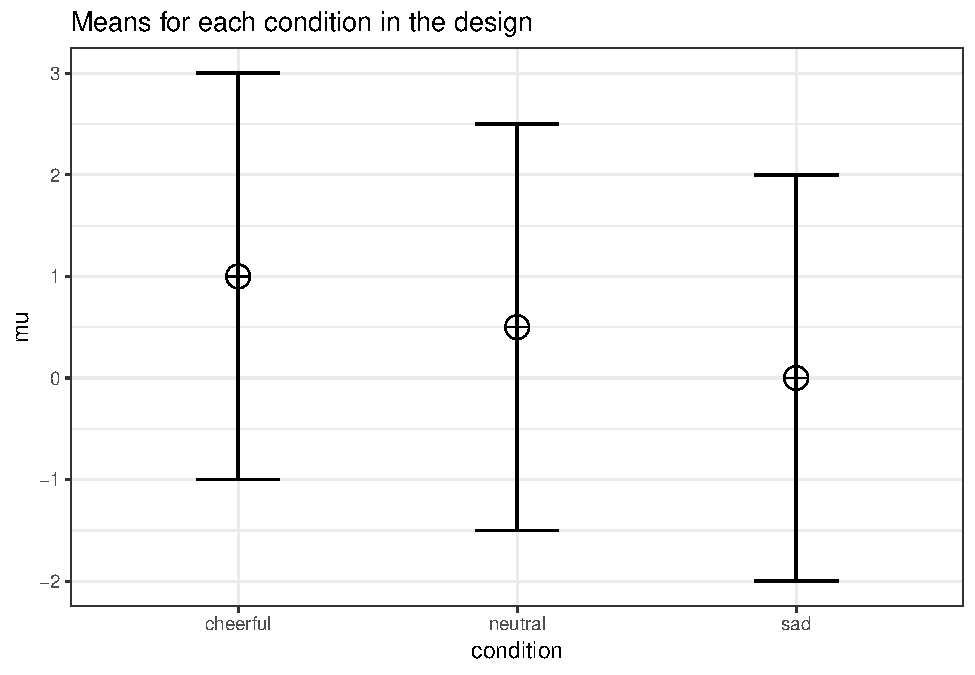
\includegraphics{4.4_power_curves_2x2_within_files/figure-latex/unnamed-chunk-5-1.pdf}

\section{Explore increase in correlation in moderated
interactions.}\label{explore-increase-in-correlation-in-moderated-interactions.}

The design has means 0, 0, 0, 0.3. The standard deviation is set to 1.
The correlation between all variables increases from 0.5 to 0.9.

\begin{Shaded}
\begin{Highlighting}[]
\NormalTok{p_a <-}\StringTok{ }\KeywordTok{plot_power_2x2_within}\NormalTok{(}\DataTypeTok{mu =} \KeywordTok{c}\NormalTok{(}\DecValTok{0}\NormalTok{,}\DecValTok{0}\NormalTok{,}\DecValTok{0}\NormalTok{,}\FloatTok{0.3}\NormalTok{), }
                      \DataTypeTok{m_A =} \DecValTok{2}\NormalTok{, }
                      \DataTypeTok{m_B =} \DecValTok{2}\NormalTok{, }
                      \DataTypeTok{sigma =} \DecValTok{1}\NormalTok{, }
                      \DataTypeTok{rho_A =} \FloatTok{0.1}\NormalTok{, }
                      \DataTypeTok{rho_B =} \FloatTok{0.1}\NormalTok{, }
                      \DataTypeTok{rho_AB =} \FloatTok{0.1}\NormalTok{, }
                      \DataTypeTok{alpha =} \FloatTok{0.05}\NormalTok{,}
\NormalTok{                      max_n <-}\StringTok{ }\DecValTok{100}\NormalTok{)}

\NormalTok{p_b <-}\StringTok{ }\KeywordTok{plot_power_2x2_within}\NormalTok{(}\DataTypeTok{mu =} \KeywordTok{c}\NormalTok{(}\DecValTok{0}\NormalTok{,}\DecValTok{0}\NormalTok{,}\DecValTok{0}\NormalTok{,}\FloatTok{0.3}\NormalTok{), }
                      \DataTypeTok{m_A =} \DecValTok{2}\NormalTok{, }
                      \DataTypeTok{m_B =} \DecValTok{2}\NormalTok{, }
                      \DataTypeTok{sigma =} \DecValTok{1}\NormalTok{, }
                      \DataTypeTok{rho_A =} \FloatTok{0.3}\NormalTok{, }
                      \DataTypeTok{rho_B =} \FloatTok{0.3}\NormalTok{, }
                      \DataTypeTok{rho_AB =} \FloatTok{0.3}\NormalTok{, }
                      \DataTypeTok{alpha =} \FloatTok{0.05}\NormalTok{,}
\NormalTok{                      max_n <-}\StringTok{ }\DecValTok{100}\NormalTok{)}

\NormalTok{p_c <-}\StringTok{ }\KeywordTok{plot_power_2x2_within}\NormalTok{(}\DataTypeTok{mu =} \KeywordTok{c}\NormalTok{(}\DecValTok{0}\NormalTok{,}\DecValTok{0}\NormalTok{,}\DecValTok{0}\NormalTok{,}\FloatTok{0.3}\NormalTok{), }
                      \DataTypeTok{m_A =} \DecValTok{2}\NormalTok{, }
                      \DataTypeTok{m_B =} \DecValTok{2}\NormalTok{, }
                      \DataTypeTok{sigma =} \DecValTok{1}\NormalTok{, }
                      \DataTypeTok{rho_A =} \FloatTok{0.5}\NormalTok{, }
                      \DataTypeTok{rho_B =} \FloatTok{0.5}\NormalTok{, }
                      \DataTypeTok{rho_AB =} \FloatTok{0.5}\NormalTok{, }
                      \DataTypeTok{alpha =} \FloatTok{0.05}\NormalTok{,}
\NormalTok{                      max_n <-}\StringTok{ }\DecValTok{100}\NormalTok{)}

\NormalTok{p_d <-}\StringTok{ }\KeywordTok{plot_power_2x2_within}\NormalTok{(}\DataTypeTok{mu =} \KeywordTok{c}\NormalTok{(}\DecValTok{0}\NormalTok{,}\DecValTok{0}\NormalTok{,}\DecValTok{0}\NormalTok{,}\FloatTok{0.3}\NormalTok{), }
                      \DataTypeTok{m_A =} \DecValTok{2}\NormalTok{, }
                      \DataTypeTok{m_B =} \DecValTok{2}\NormalTok{, }
                      \DataTypeTok{sigma =} \DecValTok{1}\NormalTok{, }
                      \DataTypeTok{rho_A =} \FloatTok{0.7}\NormalTok{, }
                      \DataTypeTok{rho_B =} \FloatTok{0.7}\NormalTok{, }
                      \DataTypeTok{rho_AB =} \FloatTok{0.7}\NormalTok{, }
                      \DataTypeTok{alpha =} \FloatTok{0.05}\NormalTok{,}
\NormalTok{                      max_n <-}\StringTok{ }\DecValTok{100}\NormalTok{)}

\NormalTok{p_e <-}\StringTok{ }\KeywordTok{plot_power_2x2_within}\NormalTok{(}\DataTypeTok{mu =} \KeywordTok{c}\NormalTok{(}\DecValTok{0}\NormalTok{,}\DecValTok{0}\NormalTok{,}\DecValTok{0}\NormalTok{,}\FloatTok{0.3}\NormalTok{), }
                      \DataTypeTok{m_A =} \DecValTok{2}\NormalTok{, }
                      \DataTypeTok{m_B =} \DecValTok{2}\NormalTok{, }
                      \DataTypeTok{sigma =} \DecValTok{1}\NormalTok{, }
                      \DataTypeTok{rho_A =} \FloatTok{0.9}\NormalTok{, }
                      \DataTypeTok{rho_B =} \FloatTok{0.9}\NormalTok{, }
                      \DataTypeTok{rho_AB =} \FloatTok{0.9}\NormalTok{, }
                      \DataTypeTok{alpha =} \FloatTok{0.05}\NormalTok{,}
\NormalTok{                      max_n <-}\StringTok{ }\DecValTok{100}\NormalTok{)}

\NormalTok{p_f <-}\StringTok{ }\KeywordTok{plot_power_2x2_within}\NormalTok{(}\DataTypeTok{mu =} \KeywordTok{c}\NormalTok{(}\DecValTok{0}\NormalTok{,}\DecValTok{0}\NormalTok{,}\DecValTok{0}\NormalTok{,}\FloatTok{0.3}\NormalTok{), }
                      \DataTypeTok{m_A =} \DecValTok{2}\NormalTok{, }
                      \DataTypeTok{m_B =} \DecValTok{2}\NormalTok{, }
                      \DataTypeTok{sigma =} \DecValTok{1}\NormalTok{, }
                      \DataTypeTok{rho_A =} \FloatTok{0.5}\NormalTok{, }
                      \DataTypeTok{rho_B =} \FloatTok{0.5}\NormalTok{, }
                      \DataTypeTok{rho_AB =} \FloatTok{0.5}\NormalTok{, }
                      \DataTypeTok{alpha =} \FloatTok{0.05}\NormalTok{,}
\NormalTok{                      max_n <-}\StringTok{ }\DecValTok{100}\NormalTok{)}

\CommentTok{# Create long format dataframe }
\NormalTok{zzz <-}\StringTok{ }\KeywordTok{rbind}\NormalTok{(p_a}\OperatorTok{$}\NormalTok{power_df, p_b}\OperatorTok{$}\NormalTok{power_df, p_c}\OperatorTok{$}\NormalTok{power_df, p_d}\OperatorTok{$}\NormalTok{power_df, p_e}\OperatorTok{$}\NormalTok{power_df, p_f}\OperatorTok{$}\NormalTok{power_df)}
\NormalTok{zzz <-}\StringTok{ }\KeywordTok{cbind}\NormalTok{(zzz,}\KeywordTok{seq}\NormalTok{(}\DecValTok{1}\NormalTok{,}\KeywordTok{length}\NormalTok{(zzz}\OperatorTok{$}\NormalTok{design)))}
\KeywordTok{colnames}\NormalTok{(zzz)[}\DecValTok{1}\NormalTok{] <-}\StringTok{ "design"}
\KeywordTok{colnames}\NormalTok{(zzz)[}\DecValTok{6}\NormalTok{] <-}\StringTok{ "ID"}
\NormalTok{zzz <-}\StringTok{ }\KeywordTok{melt}\NormalTok{(zzz, }\DataTypeTok{id.vars =} \KeywordTok{c}\NormalTok{(}\StringTok{"ID"}\NormalTok{, }\StringTok{"design"}\NormalTok{, }\StringTok{"n_vec"}\NormalTok{), }\DataTypeTok{measure.vars =} \KeywordTok{c}\NormalTok{(}\StringTok{"power_A"}\NormalTok{, }\StringTok{"power_B"}\NormalTok{, }\StringTok{"power_AB"}\NormalTok{))}

\CommentTok{# Plot data using facets, split by factors and interaction, and design}
\KeywordTok{ggplot}\NormalTok{(}\DataTypeTok{data=}\NormalTok{zzz, }\KeywordTok{aes}\NormalTok{(}\DataTypeTok{x =}\NormalTok{ n_vec, }\DataTypeTok{y =}\NormalTok{ value)) }\OperatorTok{+}
\StringTok{  }\KeywordTok{geom_line}\NormalTok{( }\DataTypeTok{size=}\FloatTok{1.5}\NormalTok{) }\OperatorTok{+}
\StringTok{  }\KeywordTok{scale_x_continuous}\NormalTok{(}\DataTypeTok{limits =} \KeywordTok{c}\NormalTok{(}\DecValTok{0}\NormalTok{, }\KeywordTok{max}\NormalTok{(zzz}\OperatorTok{$}\NormalTok{n_vec))) }\OperatorTok{+}\StringTok{ }
\StringTok{  }\KeywordTok{scale_y_continuous}\NormalTok{(}\DataTypeTok{limits =} \KeywordTok{c}\NormalTok{(}\DecValTok{0}\NormalTok{, }\DecValTok{100}\NormalTok{)) }\OperatorTok{+}
\StringTok{  }\KeywordTok{theme_bw}\NormalTok{() }\OperatorTok{+}
\StringTok{  }\KeywordTok{labs}\NormalTok{(}\DataTypeTok{x=}\StringTok{"Sample size"}\NormalTok{, }\DataTypeTok{y =} \StringTok{"Power"}\NormalTok{) }\OperatorTok{+}
\StringTok{  }\KeywordTok{facet_grid}\NormalTok{(design}\OperatorTok{~}\NormalTok{variable)}
\end{Highlighting}
\end{Shaded}

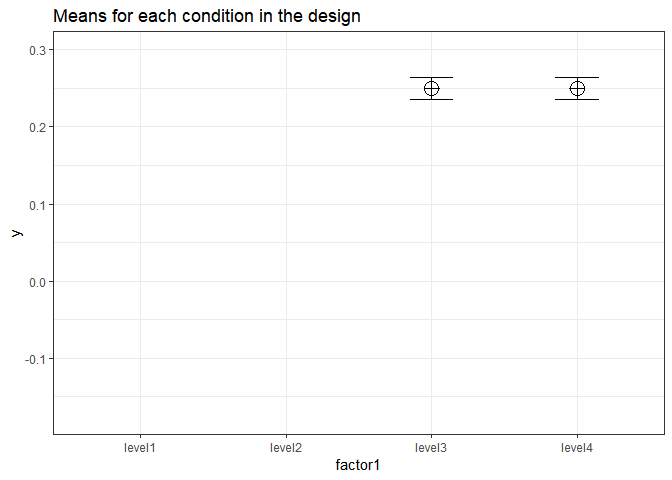
\includegraphics{4.4_power_curves_2x2_within_files/figure-latex/unnamed-chunk-6-1.pdf}

\section{Increasing correlation in on factor decreases power in second
factor}\label{increasing-correlation-in-on-factor-decreases-power-in-second-factor}

As Potvin and Schutz (2000) write: ``The more important finding with
respect to the effect of \emph{r} on power relates to the effect of the
correlations associated with one factor on the power of the test of the
main effect of the other factor. Specifically, if the correlations among
the levels of B are larger than those within the AB matrix (i.e.,
\emph{r}B - \emph{r}AB \textgreater{} 0.0), there is a reduction in the
power for the test of the A effect (and the test on B is similarly
affected by the A correlations).''

We see this in the plots below. As the correlation of the A factor
increases from 0.4 to 0.9, we see the power for the main effect of
factor B decreases.

\begin{Shaded}
\begin{Highlighting}[]
\NormalTok{p_a <-}\StringTok{ }\KeywordTok{plot_power_2x2_within}\NormalTok{(}\DataTypeTok{mu =} \KeywordTok{c}\NormalTok{(}\DecValTok{0}\NormalTok{,}\DecValTok{0}\NormalTok{,}\DecValTok{0}\NormalTok{,}\FloatTok{0.3}\NormalTok{), }
                      \DataTypeTok{m_A =} \DecValTok{2}\NormalTok{, }
                      \DataTypeTok{m_B =} \DecValTok{2}\NormalTok{, }
                      \DataTypeTok{sigma =} \DecValTok{1}\NormalTok{, }
                      \DataTypeTok{rho_A =} \FloatTok{0.4}\NormalTok{, }
                      \DataTypeTok{rho_B =} \FloatTok{0.4}\NormalTok{, }
                      \DataTypeTok{rho_AB =} \FloatTok{0.4}\NormalTok{, }
                      \DataTypeTok{alpha =} \FloatTok{0.05}\NormalTok{,}
\NormalTok{                      max_n <-}\StringTok{ }\DecValTok{100}\NormalTok{)}

\NormalTok{p_b <-}\StringTok{ }\KeywordTok{plot_power_2x2_within}\NormalTok{(}\DataTypeTok{mu =} \KeywordTok{c}\NormalTok{(}\DecValTok{0}\NormalTok{,}\DecValTok{0}\NormalTok{,}\DecValTok{0}\NormalTok{,}\FloatTok{0.3}\NormalTok{), }
                      \DataTypeTok{m_A =} \DecValTok{2}\NormalTok{, }
                      \DataTypeTok{m_B =} \DecValTok{2}\NormalTok{, }
                      \DataTypeTok{sigma =} \DecValTok{1}\NormalTok{, }
                      \DataTypeTok{rho_A =} \FloatTok{0.5}\NormalTok{, }
                      \DataTypeTok{rho_B =} \FloatTok{0.4}\NormalTok{, }
                      \DataTypeTok{rho_AB =} \FloatTok{0.4}\NormalTok{, }
                      \DataTypeTok{alpha =} \FloatTok{0.05}\NormalTok{,}
\NormalTok{                      max_n <-}\StringTok{ }\DecValTok{100}\NormalTok{)}

\NormalTok{p_c <-}\StringTok{ }\KeywordTok{plot_power_2x2_within}\NormalTok{(}\DataTypeTok{mu =} \KeywordTok{c}\NormalTok{(}\DecValTok{0}\NormalTok{,}\DecValTok{0}\NormalTok{,}\DecValTok{0}\NormalTok{,}\FloatTok{0.3}\NormalTok{), }
                      \DataTypeTok{m_A =} \DecValTok{2}\NormalTok{, }
                      \DataTypeTok{m_B =} \DecValTok{2}\NormalTok{, }
                      \DataTypeTok{sigma =} \DecValTok{1}\NormalTok{, }
                      \DataTypeTok{rho_A =} \FloatTok{0.6}\NormalTok{, }
                      \DataTypeTok{rho_B =} \FloatTok{0.4}\NormalTok{, }
                      \DataTypeTok{rho_AB =} \FloatTok{0.4}\NormalTok{, }
                      \DataTypeTok{alpha =} \FloatTok{0.05}\NormalTok{,}
\NormalTok{                      max_n <-}\StringTok{ }\DecValTok{100}\NormalTok{)}

\NormalTok{p_d <-}\StringTok{ }\KeywordTok{plot_power_2x2_within}\NormalTok{(}\DataTypeTok{mu =} \KeywordTok{c}\NormalTok{(}\DecValTok{0}\NormalTok{,}\DecValTok{0}\NormalTok{,}\DecValTok{0}\NormalTok{,}\FloatTok{0.3}\NormalTok{), }
                      \DataTypeTok{m_A =} \DecValTok{2}\NormalTok{, }
                      \DataTypeTok{m_B =} \DecValTok{2}\NormalTok{, }
                      \DataTypeTok{sigma =} \DecValTok{1}\NormalTok{, }
                      \DataTypeTok{rho_A =} \FloatTok{0.7}\NormalTok{, }
                      \DataTypeTok{rho_B =} \FloatTok{0.4}\NormalTok{, }
                      \DataTypeTok{rho_AB =} \FloatTok{0.4}\NormalTok{, }
                      \DataTypeTok{alpha =} \FloatTok{0.05}\NormalTok{,}
\NormalTok{                      max_n <-}\StringTok{ }\DecValTok{100}\NormalTok{)}

\NormalTok{p_e <-}\StringTok{ }\KeywordTok{plot_power_2x2_within}\NormalTok{(}\DataTypeTok{mu =} \KeywordTok{c}\NormalTok{(}\DecValTok{0}\NormalTok{,}\DecValTok{0}\NormalTok{,}\DecValTok{0}\NormalTok{,}\FloatTok{0.3}\NormalTok{), }
                      \DataTypeTok{m_A =} \DecValTok{2}\NormalTok{, }
                      \DataTypeTok{m_B =} \DecValTok{2}\NormalTok{, }
                      \DataTypeTok{sigma =} \DecValTok{1}\NormalTok{, }
                      \DataTypeTok{rho_A =} \FloatTok{0.8}\NormalTok{, }
                      \DataTypeTok{rho_B =} \FloatTok{0.4}\NormalTok{, }
                      \DataTypeTok{rho_AB =} \FloatTok{0.4}\NormalTok{, }
                      \DataTypeTok{alpha =} \FloatTok{0.05}\NormalTok{,}
\NormalTok{                      max_n <-}\StringTok{ }\DecValTok{100}\NormalTok{)}

\NormalTok{p_f <-}\StringTok{ }\KeywordTok{plot_power_2x2_within}\NormalTok{(}\DataTypeTok{mu =} \KeywordTok{c}\NormalTok{(}\DecValTok{0}\NormalTok{,}\DecValTok{0}\NormalTok{,}\DecValTok{0}\NormalTok{,}\FloatTok{0.3}\NormalTok{), }
                      \DataTypeTok{m_A =} \DecValTok{2}\NormalTok{, }
                      \DataTypeTok{m_B =} \DecValTok{2}\NormalTok{, }
                      \DataTypeTok{sigma =} \DecValTok{1}\NormalTok{, }
                      \DataTypeTok{rho_A =} \FloatTok{0.9}\NormalTok{, }
                      \DataTypeTok{rho_B =} \FloatTok{0.4}\NormalTok{, }
                      \DataTypeTok{rho_AB =} \FloatTok{0.4}\NormalTok{, }
                      \DataTypeTok{alpha =} \FloatTok{0.05}\NormalTok{,}
\NormalTok{                      max_n <-}\StringTok{ }\DecValTok{100}\NormalTok{)}

\CommentTok{# Create long format dataframe }
\NormalTok{zzz <-}\StringTok{ }\KeywordTok{rbind}\NormalTok{(p_a}\OperatorTok{$}\NormalTok{power_df, p_b}\OperatorTok{$}\NormalTok{power_df, p_c}\OperatorTok{$}\NormalTok{power_df, p_d}\OperatorTok{$}\NormalTok{power_df, p_e}\OperatorTok{$}\NormalTok{power_df, p_f}\OperatorTok{$}\NormalTok{power_df)}
\NormalTok{zzz <-}\StringTok{ }\KeywordTok{cbind}\NormalTok{(zzz,}\KeywordTok{seq}\NormalTok{(}\DecValTok{1}\NormalTok{,}\KeywordTok{length}\NormalTok{(zzz}\OperatorTok{$}\NormalTok{design)))}
\KeywordTok{colnames}\NormalTok{(zzz)[}\DecValTok{1}\NormalTok{] <-}\StringTok{ "design"}
\KeywordTok{colnames}\NormalTok{(zzz)[}\DecValTok{6}\NormalTok{] <-}\StringTok{ "ID"}
\NormalTok{zzz <-}\StringTok{ }\KeywordTok{melt}\NormalTok{(zzz, }\DataTypeTok{id.vars =} \KeywordTok{c}\NormalTok{(}\StringTok{"ID"}\NormalTok{, }\StringTok{"design"}\NormalTok{, }\StringTok{"n_vec"}\NormalTok{), }\DataTypeTok{measure.vars =} \KeywordTok{c}\NormalTok{(}\StringTok{"power_A"}\NormalTok{, }\StringTok{"power_B"}\NormalTok{, }\StringTok{"power_AB"}\NormalTok{))}

\CommentTok{# Plot data using facets, split by factors and interaction, and design}
\KeywordTok{ggplot}\NormalTok{(}\DataTypeTok{data=}\NormalTok{zzz, }\KeywordTok{aes}\NormalTok{(}\DataTypeTok{x =}\NormalTok{ n_vec, }\DataTypeTok{y =}\NormalTok{ value)) }\OperatorTok{+}
\StringTok{  }\KeywordTok{geom_line}\NormalTok{( }\DataTypeTok{size=}\FloatTok{1.5}\NormalTok{) }\OperatorTok{+}
\StringTok{  }\KeywordTok{scale_x_continuous}\NormalTok{(}\DataTypeTok{limits =} \KeywordTok{c}\NormalTok{(}\DecValTok{0}\NormalTok{, }\KeywordTok{max}\NormalTok{(zzz}\OperatorTok{$}\NormalTok{n_vec))) }\OperatorTok{+}\StringTok{ }
\StringTok{  }\KeywordTok{scale_y_continuous}\NormalTok{(}\DataTypeTok{limits =} \KeywordTok{c}\NormalTok{(}\DecValTok{0}\NormalTok{, }\DecValTok{100}\NormalTok{)) }\OperatorTok{+}
\StringTok{  }\KeywordTok{theme_bw}\NormalTok{() }\OperatorTok{+}
\StringTok{  }\KeywordTok{labs}\NormalTok{(}\DataTypeTok{x=}\StringTok{"Sample size"}\NormalTok{, }\DataTypeTok{y =} \StringTok{"Power"}\NormalTok{) }\OperatorTok{+}
\StringTok{  }\KeywordTok{facet_grid}\NormalTok{(design}\OperatorTok{~}\NormalTok{variable)}
\end{Highlighting}
\end{Shaded}

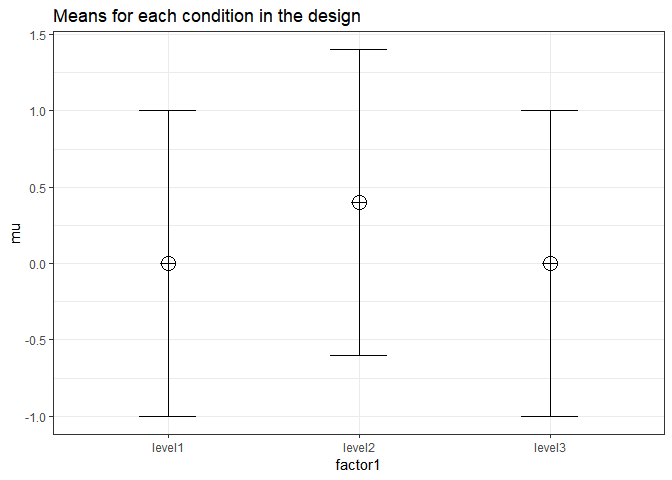
\includegraphics{4.4_power_curves_2x2_within_files/figure-latex/unnamed-chunk-7-1.pdf}


\end{document}
